\section{\textbf{ДОПОЛНИТЕЛЬНАЯ ГЛАВА ДЛЯ СИТ}}

Это дополнительная глава, которая не несет смысловой нагрузки для главной темы реферата. Здесь я покажу некоторые полезные фишки Latex, которые помогает мне в учебе.

Для начало стоит определиться с задачами, а именно, что мы можем использовать:
\begin{itemize}
    \item Вставка файла (уже сделали)
    \item Нумерованные и маркерованные списки (уже сделали)
    \item Список источников (уже готово)
    \item Вставка изображений
    \item Вставка таблиц
    \item Формулы
    \item Программный код, с помощью minted
\end{itemize}

\subsection{Вставка изображений}
Первое с чего я начну, это вставка изобржений, мы можем менять размер, сентрировать ее и изменить описание.

\begin{figure}[H]
\centering
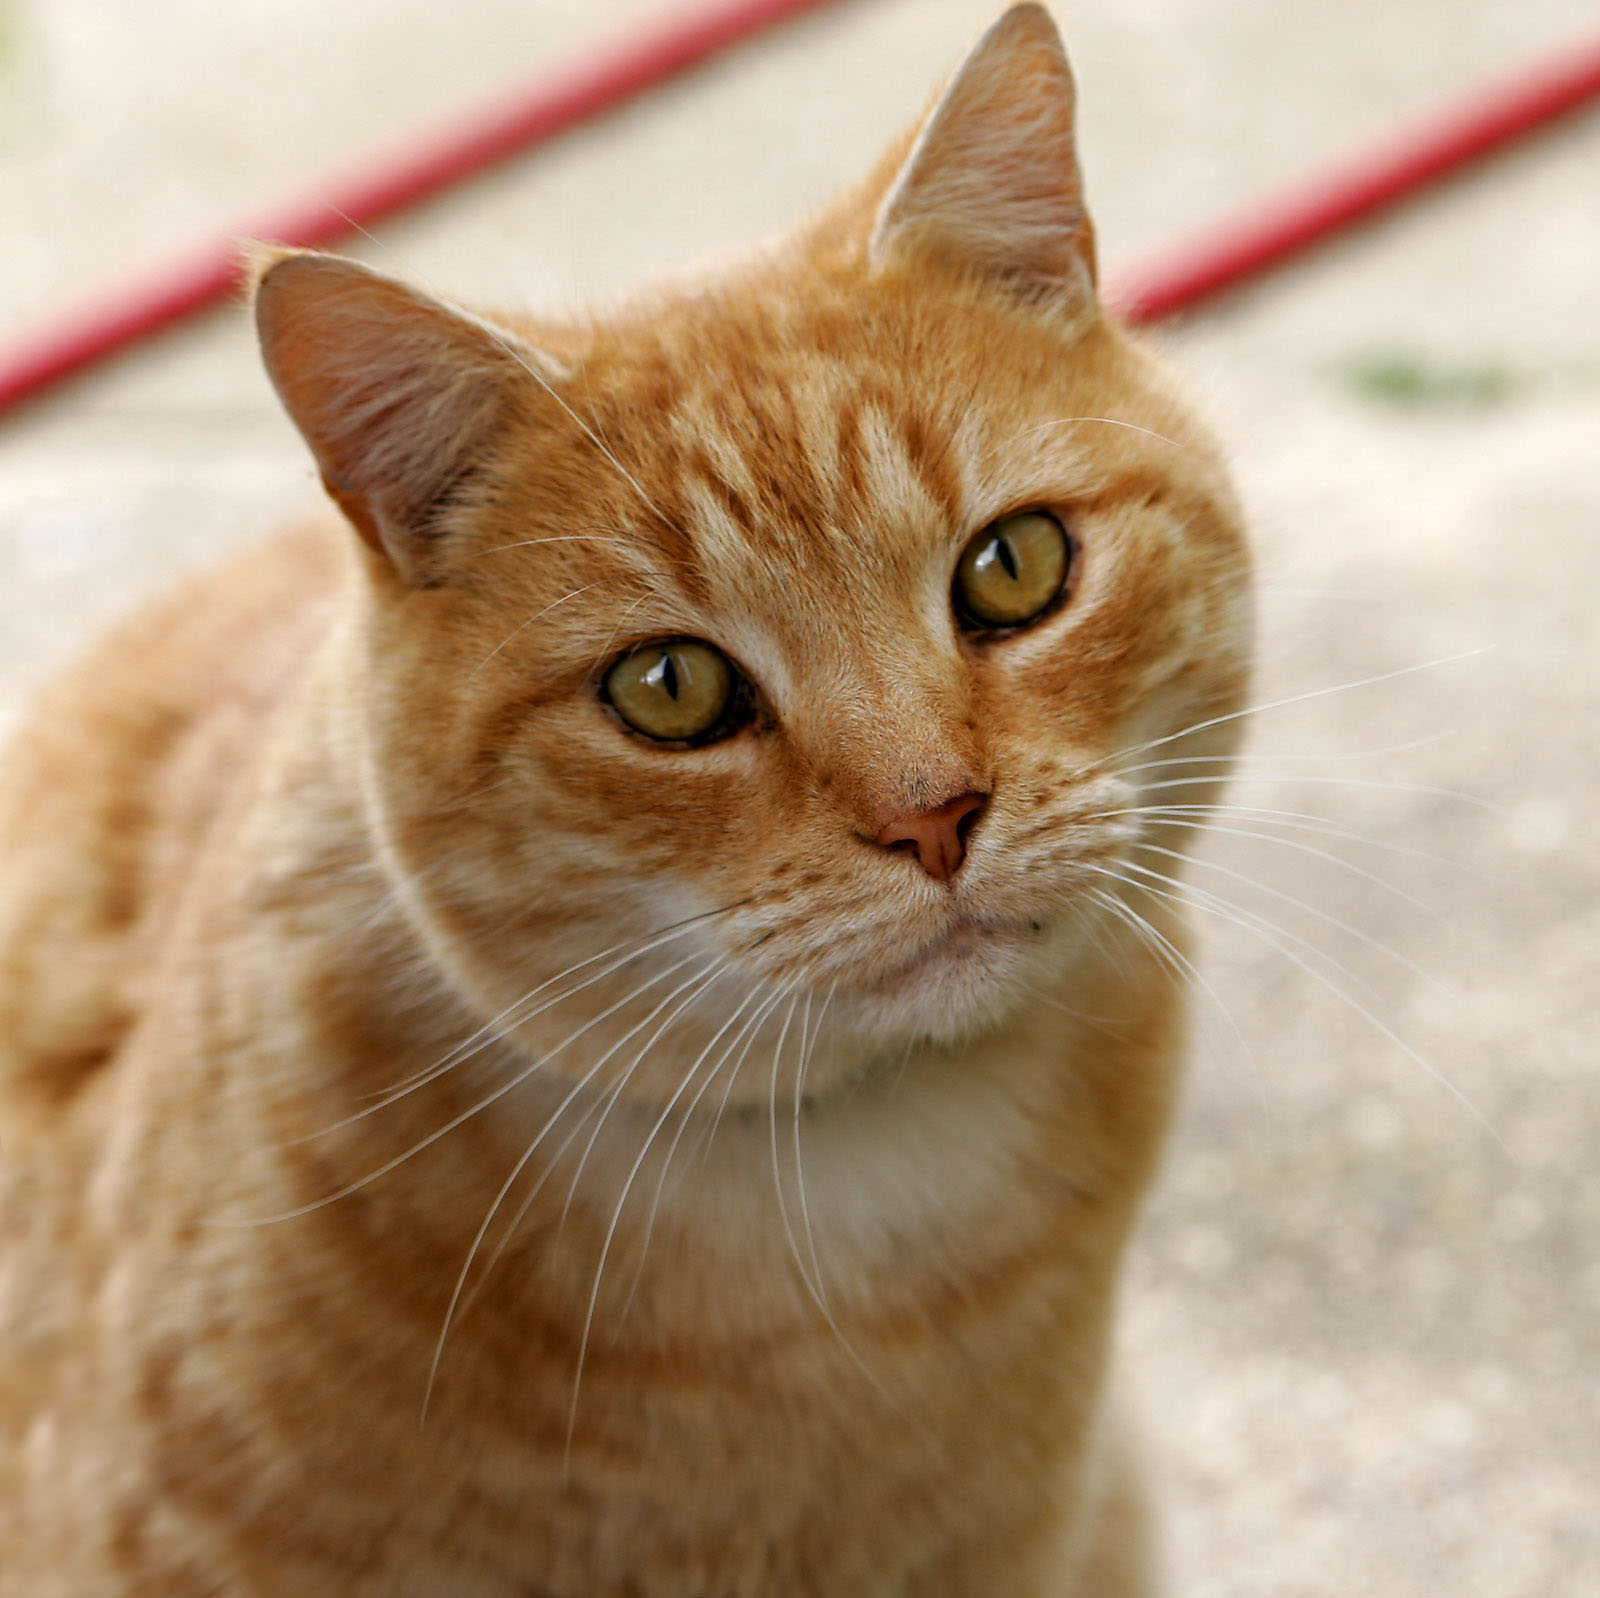
\includegraphics[width=0.5\linewidth]{cat.jpeg}
\caption{\label{fig:cat}Рыжий кот по центру.}
\end{figure}

Также можно вставлять сразу несколько изображений:
\begin{figure}[H]
\centering

\includegraphics[width=0.5\linewidth]{cat1.jpeg}
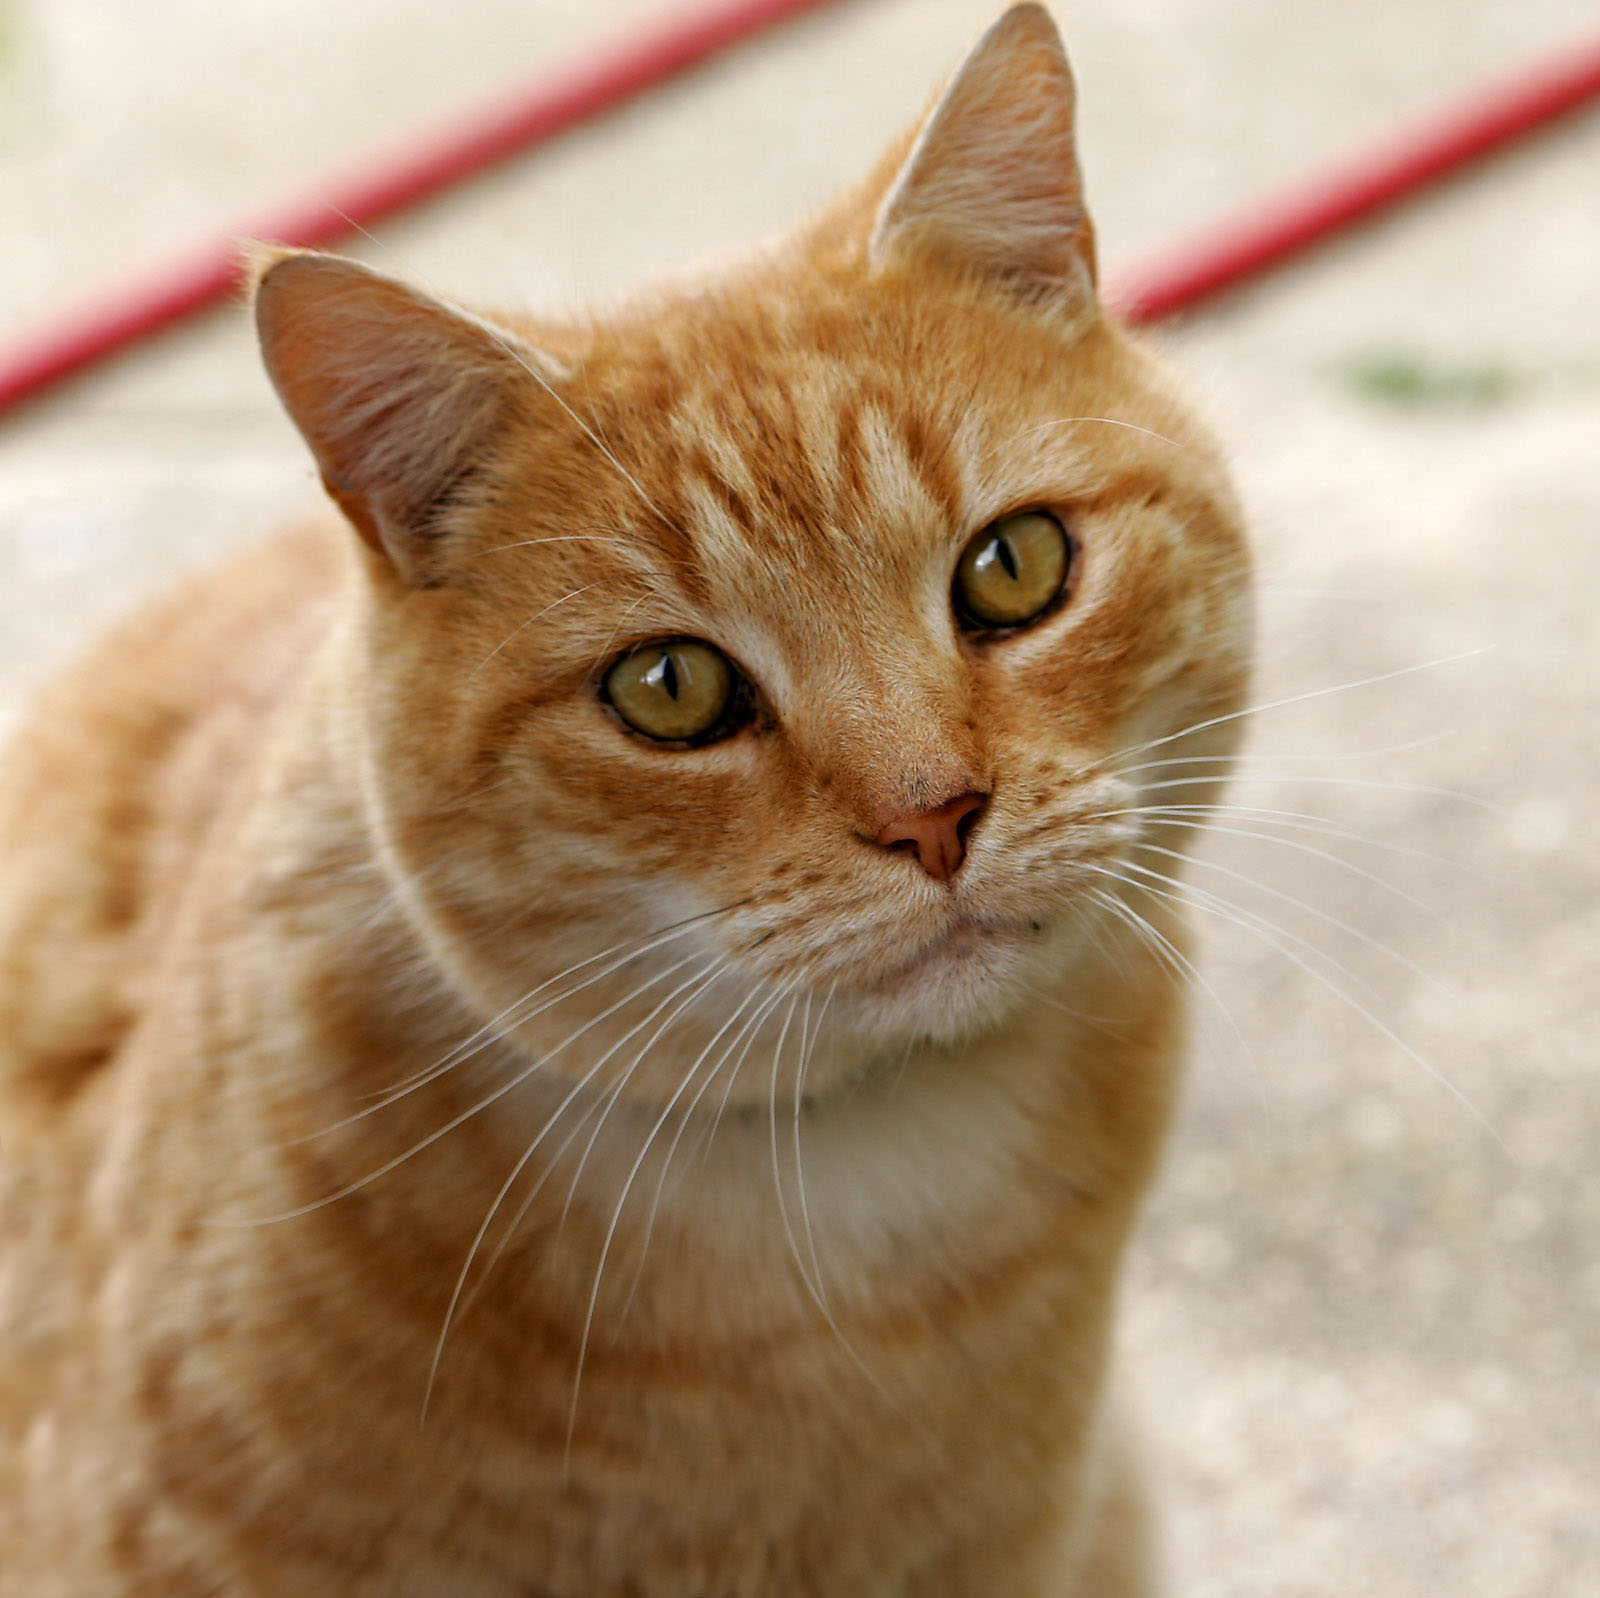
\includegraphics[width=0.3\linewidth]{cat.jpeg}
\caption{\label{fig:cat}Два кота по центру.}
\end{figure}

\subsection{Таблицы}

Таблицы всегда играют важную роль в рефератах, докладах и так далее. Их можно сделать и здесь:
\begin{table}[h]
    \centering
    \begin{tabular}{|c|c|c|}
        \hline
        Header 1 & Header 2 & Header 3 \\
        \hline
        Row 1, Column 1 & Row 1, Column 2 & Row 1, Column 3 \\
        Row 2, Column 1 & Row 2, Column 2 & Row 2, Column 3 \\
        Row 3, Column 1 & Row 3, Column 2 & Row 3, Column 3 \\
        Row 4, Column 1 & Row 4, Column 2 & Row 4, Column 3 \\
        Row 5, Column 1 & Row 5, Column 2 & Row 5, Column 3 \\
        \hline
    \end{tabular}
\end{table}

Чем то похоже на запись матрицы:
\[
\begin{bmatrix}
a & b & c \\
d & e & f \\
g & h & i \\
\end{bmatrix}
\]

\subsection{Математические формулы}
На своем опыте могу сказать, что записывать лекции по матану куда практичнее здесь, но к этому нужно еще привыкнуть.

\subsubsection{Инлайн-формулы}
Первое с чего стоит начать, это с использования инлайн формул: $f(x)=x_0 x_0 + x_1 a_1^2$

\subsubsection{Выносные формулы}
Дальше идут выносные формулы, на которые удобно ссылаться: 
\begin{equation}
    \frac{x-y}{a+b}
    \label{eq: formula}
\end{equation}

Ссылаюсь на формулу \ref{eq: formula}.
В записи лекций по матану, часто могут понадобиться специальные символы, вот парочку из них: 


\begin{equation}
    \sum_{i=0}^n a_i \cdot x_i
\end{equation}
\begin{equation}
    \int_{i=0}^n a_i \cdot x_i
\end{equation}
\begin{equation}
    \prod_{i=0}^n a_i \cdot x_i
\end{equation}

\subsection{Программный код}
Часто может понадобиться использовать код со своих программ в некоторых рефератах, это возможно сделать с помощью minted. Рассмотрим пример с базовой программой вывода \mintinline{c++}|"Hello, world!"|

\begin{listing}[H]
    \caption{Hello world in c++}
    \begin{minted}{c++}
#include <iostream>
int main() {
    std::cout << "Hello world" << std::endl;
    return 0;
}
    \end{minted}
\end{listing}

\subsection{Мини вывод}

После использования LaTeX я выявел некоторые плюсы:

1. Качественное оформление документов: LaTeX позволяет создавать профессионально оформленные документы с помощью различных шаблонов, стилей и форматирования.

2. Математические формулы: LaTeX имеет специальные команды для ввода сложных математических формул, что делает его идеальным инструментом для написания научных статей и докладов.

3. Удобство работы с большими документами: LaTeX автоматически нумерует главы, разделы, таблицы и изображения, упрощая процесс создания и редактирования больших документов.

4. Кроссплатформенность: LaTeX работает на различных операционных системах, включая Windows, macOS и Linux, что делает его удобным для совместной работы над проектами.

5. Бесплатность: LaTeX является свободным программным обеспечением, доступным для скачивания и использования без ограничений.

6. Широкие возможности настройки: LaTeX позволяет настраивать различные аспекты документа, такие как шрифты, отступы, межстрочные интервалы и многое другое, для создания уникального и оригинального оформления.
